\documentclass[tikz,12pt,border=2pt]{standalone}
\usepackage[T1]{fontenc}
\usetikzlibrary{arrows.meta,shapes.geometric}
\definecolor{accent}{RGB}{31,84,140}
\definecolor{accentlight}{RGB}{200,214,232}
\begin{document}
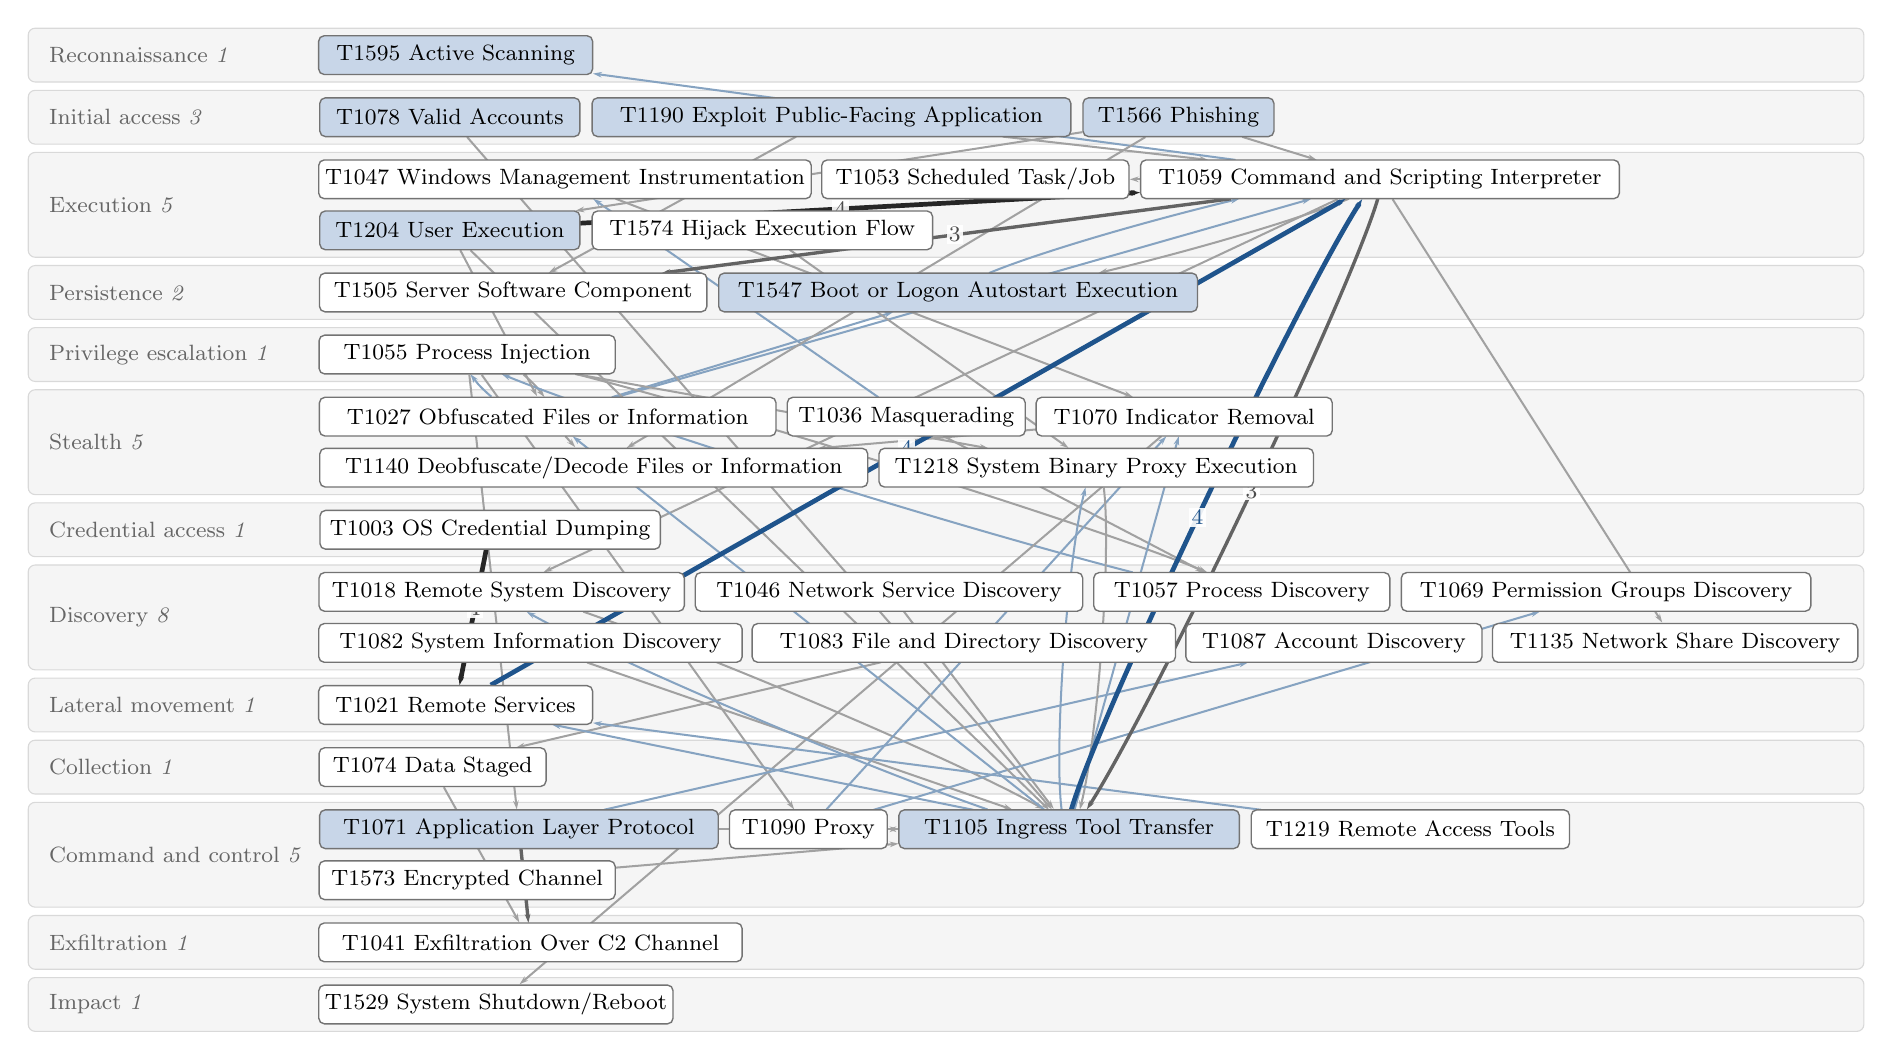
\begin{tikzpicture}[x=1pt,y=1pt]
\draw[rounded corners=2.50pt,draw=black!15,fill=black!4,line width=0.40pt] (-104.94,340.32) rectangle (558.37,359.76);
\node[anchor=west,text=black!60,align=left,font=\fontsize{8.00}{9.20}\selectfont] at (-100.94,350.04) {Reconnaissance\,\,{\itshape 1}};
\draw[rounded corners=2.50pt,draw=black!15,fill=black!4,line width=0.40pt] (-104.94,317.88) rectangle (558.37,337.32);
\node[anchor=west,text=black!60,align=left,font=\fontsize{8.00}{9.20}\selectfont] at (-100.94,327.60) {Initial access\,\,{\itshape 3}};
\draw[rounded corners=2.50pt,draw=black!15,fill=black!4,line width=0.40pt] (-104.94,277.00) rectangle (558.37,314.88);
\node[anchor=west,text=black!60,align=left,font=\fontsize{8.00}{9.20}\selectfont] at (-100.94,295.94) {Execution\,\,{\itshape 5}};
\draw[rounded corners=2.50pt,draw=black!15,fill=black!4,line width=0.40pt] (-104.94,254.56) rectangle (558.37,274.00);
\node[anchor=west,text=black!60,align=left,font=\fontsize{8.00}{9.20}\selectfont] at (-100.94,264.28) {Persistence\,\,{\itshape 2}};
\draw[rounded corners=2.50pt,draw=black!15,fill=black!4,line width=0.40pt] (-104.94,232.12) rectangle (558.37,251.56);
\node[anchor=west,text=black!60,align=left,font=\fontsize{8.00}{9.20}\selectfont] at (-100.94,241.84) {Privilege escalation\,\,{\itshape 1}};
\draw[rounded corners=2.50pt,draw=black!15,fill=black!4,line width=0.40pt] (-104.94,191.24) rectangle (558.37,229.12);
\node[anchor=west,text=black!60,align=left,font=\fontsize{8.00}{9.20}\selectfont] at (-100.94,210.18) {Stealth\,\,{\itshape 5}};
\draw[rounded corners=2.50pt,draw=black!15,fill=black!4,line width=0.40pt] (-104.94,168.80) rectangle (558.37,188.24);
\node[anchor=west,text=black!60,align=left,font=\fontsize{8.00}{9.20}\selectfont] at (-100.94,178.52) {Credential access\,\,{\itshape 1}};
\draw[rounded corners=2.50pt,draw=black!15,fill=black!4,line width=0.40pt] (-104.94,127.92) rectangle (558.37,165.80);
\node[anchor=west,text=black!60,align=left,font=\fontsize{8.00}{9.20}\selectfont] at (-100.94,146.86) {Discovery\,\,{\itshape 8}};
\draw[rounded corners=2.50pt,draw=black!15,fill=black!4,line width=0.40pt] (-104.94,105.48) rectangle (558.37,124.92);
\node[anchor=west,text=black!60,align=left,font=\fontsize{8.00}{9.20}\selectfont] at (-100.94,115.20) {Lateral movement\,\,{\itshape 1}};
\draw[rounded corners=2.50pt,draw=black!15,fill=black!4,line width=0.40pt] (-104.94,83.04) rectangle (558.37,102.48);
\node[anchor=west,text=black!60,align=left,font=\fontsize{8.00}{9.20}\selectfont] at (-100.94,92.76) {Collection\,\,{\itshape 1}};
\draw[rounded corners=2.50pt,draw=black!15,fill=black!4,line width=0.40pt] (-104.94,42.16) rectangle (558.37,80.04);
\node[anchor=west,text=black!60,align=left,font=\fontsize{8.00}{9.20}\selectfont] at (-100.94,61.10) {Command and control\,\,{\itshape 5}};
\draw[rounded corners=2.50pt,draw=black!15,fill=black!4,line width=0.40pt] (-104.94,19.72) rectangle (558.37,39.16);
\node[anchor=west,text=black!60,align=left,font=\fontsize{8.00}{9.20}\selectfont] at (-100.94,29.44) {Exfiltration\,\,{\itshape 1}};
\draw[rounded corners=2.50pt,draw=black!15,fill=black!4,line width=0.40pt] (-104.94,-2.72) rectangle (558.37,16.72);
\node[anchor=west,text=black!60,align=left,font=\fontsize{8.00}{9.20}\selectfont] at (-100.94,7.00) {Impact\,\,{\itshape 1}};
\draw[draw=black!37,line width=0.73pt,-{Stealth[length=3.20pt,width=2.00pt]}] (95.64,148.93) .. controls (140.92,133.18) and (225.65,97.34) .. (258.11,79.77) -- (262.16,77.52);
\draw[draw=accent!54,line width=0.73pt,-{Stealth[length=3.20pt,width=2.00pt]}] (62.42,226.62) .. controls (60.66,228.09) and (59.02,229.64) .. (57.62,231.19) -- (54.83,234.76);
\draw[draw=accent!54,line width=0.73pt,-{Stealth[length=3.20pt,width=2.00pt]}] (107.39,226.42) .. controls (162.35,242.09) and (294.88,279.89) .. (354.08,296.77) -- (358.55,298.04);
\draw[draw=black!37,line width=0.73pt,-{Stealth[length=3.20pt,width=2.00pt]}] (89.17,212.32) .. controls (89.31,212.16) and (89.46,212.00) .. (89.61,211.83) -- (92.75,208.35);
\draw[draw=accent!54,line width=0.73pt,-{Stealth[length=3.20pt,width=2.00pt]}] (105.95,226.41) .. controls (132.24,234.37) and (175.09,247.34) .. (203.19,255.84) -- (207.56,257.17);
\draw[draw=accent!54,line width=0.73pt,-{Stealth[length=3.20pt,width=2.00pt]}] (202.25,226.42) .. controls (180.30,241.68) and (128.17,277.93) .. (103.04,295.41) -- (99.25,298.04);
\draw[draw=black!37,line width=0.73pt,-{Stealth[length=3.20pt,width=2.00pt]}] (225.78,212.38) .. controls (247.81,200.88) and (291.60,178.01) .. (316.04,165.24) -- (320.08,163.13);
\draw[draw=black!37,line width=0.73pt,-{Stealth[length=3.20pt,width=2.00pt]}] (211.43,149.06) .. controls (222.71,134.19) and (249.13,99.38) .. (262.74,81.44) -- (265.60,77.68);
\draw[draw=black!37,line width=0.73pt,-{Stealth[length=3.20pt,width=2.00pt]}] (107.33,298.14) .. controls (147.90,282.59) and (245.26,245.28) .. (289.82,228.20) -- (294.22,226.52);
\draw[draw=black!37,line width=0.73pt,-{Stealth[length=3.20pt,width=2.00pt]}] (74.02,234.62) .. controls (75.78,233.15) and (77.42,231.60) .. (78.83,230.05) -- (81.61,226.48);
\draw[draw=black!37,line width=0.73pt,-{Stealth[length=3.20pt,width=2.00pt]}] (93.11,234.78) .. controls (155.26,218.85) and (273.33,182.22) .. (316.90,164.85) -- (321.12,163.13);
\draw[draw=black!37,line width=0.73pt,-{Stealth[length=3.20pt,width=2.00pt]}] (54.46,234.47) .. controls (57.39,207.69) and (67.46,115.37) .. (71.08,82.26) -- (71.60,77.47);
\draw[draw=black!37,line width=0.73pt,-{Stealth[length=3.20pt,width=2.00pt]}] (58.96,234.47) .. controls (78.37,207.47) and (145.68,113.85) .. (168.98,81.45) -- (171.84,77.47);
\draw[draw=black!37,line width=0.73pt,-{Stealth[length=3.20pt,width=2.00pt]}] (92.74,234.81) .. controls (133.03,227.57) and (195.72,216.29) .. (237.55,208.77) -- (242.03,207.96);
\draw[draw=accent!54,line width=0.73pt,-{Stealth[length=3.20pt,width=2.00pt]}] (294.13,163.14) .. controls (231.98,179.07) and (113.91,215.70) .. (70.34,233.07) -- (66.12,234.79);
\draw[draw=black!37,line width=0.73pt,-{Stealth[length=3.20pt,width=2.00pt]}] (368.19,297.97) .. controls (315.82,273.37) and (143.83,192.58) .. (85.61,165.23) -- (81.29,163.20);
\draw[draw=black!37,line width=0.73pt,-{Stealth[length=3.20pt,width=2.00pt]}] (296.77,305.16) .. controls (296.61,305.16) and (296.46,305.16) .. (296.30,305.16) -- (293.09,305.16);
\draw[draw=black!37,line width=0.73pt,-{Stealth[length=3.20pt,width=2.00pt]}] (388.08,297.96) .. controls (404.80,271.71) and (462.58,180.98) .. (482.98,148.95) -- (485.49,145.00);
\draw[draw=black!37,line width=0.73pt,-{Stealth[length=3.20pt,width=2.00pt]}] (372.29,298.14) .. controls (354.28,290.72) and (317.81,280.04) .. (286.43,272.42) -- (281.84,271.32);
\draw[draw=accent!54,line width=0.73pt,-{Stealth[length=3.20pt,width=2.00pt]}] (331.31,312.17) .. controls (269.44,320.49) and (166.83,334.27) .. (103.97,342.72) -- (99.14,343.37);
\draw[draw=black!37,line width=0.73pt,-{Stealth[length=3.20pt,width=2.00pt]}] (259.22,214.77) .. controls (236.79,212.83) and (210.15,210.53) .. (185.13,208.37) -- (180.47,207.97);
\draw[draw=black!37,line width=0.73pt,-{Stealth[length=3.20pt,width=2.00pt]}] (304.50,212.33) .. controls (267.85,181.03) and (120.00,54.77) .. (76.29,17.44) -- (72.62,14.31);
\draw[draw=accent!54,line width=0.73pt,-{Stealth[length=3.20pt,width=2.00pt]}] (103.06,77.33) .. controls (158.05,89.90) and (273.07,116.20) .. (331.37,129.53) -- (335.81,130.54);
\draw[draw=black!37,line width=0.73pt,-{Stealth[length=3.20pt,width=2.00pt]}] (144.43,70.32) .. controls (164.10,70.32) and (185.32,70.32) .. (204.66,70.32) -- (209.54,70.32);
\draw[draw=black!37,line width=0.73pt,-{Stealth[length=3.20pt,width=2.00pt]}] (45.24,85.50) .. controls (51.36,74.52) and (63.03,53.63) .. (70.26,40.68) -- (72.53,36.62);
\draw[draw=black!37,line width=0.73pt,-{Stealth[length=3.20pt,width=2.00pt]}] (53.64,320.45) .. controls (84.81,284.61) and (224.08,124.47) .. (261.76,81.15) -- (264.89,77.56);
\draw[draw=black!37,line width=0.73pt,-{Stealth[length=3.20pt,width=2.00pt]}] (97.00,130.56) .. controls (132.92,118.14) and (207.20,92.45) .. (246.13,78.98) -- (250.70,77.40);
\draw[draw=black!37,line width=0.73pt,-{Stealth[length=3.20pt,width=2.00pt]}] (203.15,130.63) .. controls (168.73,122.58) and (112.39,109.41) .. (76.05,100.91) -- (71.28,99.80);
\draw[draw=accent!54,line width=0.73pt,-{Stealth[length=3.20pt,width=2.00pt]}] (200.57,77.34) .. controls (253.14,92.98) and (379.76,130.65) .. (436.68,147.59) -- (441.31,148.96);
\draw[draw=accent!54,line width=0.73pt,-{Stealth[length=3.20pt,width=2.00pt]}] (183.53,77.51) .. controls (205.54,101.67) and (276.90,180.01) .. (303.05,208.72) -- (306.30,212.28);
\draw[draw=accent!54,line width=0.73pt,-{Stealth[length=3.20pt,width=2.00pt]}] (241.68,77.47) .. controls (196.40,93.22) and (111.67,129.06) .. (79.21,146.63) -- (75.16,148.88);
\draw[draw=accent!54,line width=0.73pt,-{Stealth[length=3.20pt,width=2.00pt]}] (236.54,77.33) .. controls (196.48,85.44) and (130.67,98.77) .. (88.75,107.25) -- (84.26,108.16);
\draw[draw=accent!54,line width=0.73pt,-{Stealth[length=3.20pt,width=2.00pt]}] (262.09,77.51) .. controls (231.31,101.87) and (130.94,181.29) .. (95.40,209.42) -- (91.78,212.28);
\draw[draw=accent!54,line width=0.73pt,-{Stealth[length=3.20pt,width=2.00pt]}] (273.19,77.51) .. controls (279.85,101.37) and (301.25,178.10) .. (309.50,207.65) -- (310.79,212.28);
\draw[draw=black!37,line width=0.73pt,-{Stealth[length=3.20pt,width=2.00pt]}] (209.66,70.32) .. controls (209.57,70.32) and (209.49,70.32) .. (209.40,70.32) -- (205.53,70.32);
\draw[draw=accent!54,line width=0.73pt,-{Stealth[length=3.20pt,width=2.00pt]}] (268.45,77.59) .. controls (265.71,99.17) and (270.22,162.99) .. (276.01,189.36) -- (277.10,193.83);
\draw[draw=black!37,line width=0.73pt,-{Stealth[length=3.20pt,width=2.00pt]}] (247.20,320.59) .. controls (269.25,318.09) and (294.19,315.27) .. (316.64,312.73) -- (321.39,312.19);
\draw[draw=black!37,line width=0.73pt,-{Stealth[length=3.20pt,width=2.00pt]}] (172.55,320.58) .. controls (151.74,309.12) and (110.47,286.40) .. (87.22,273.60) -- (83.10,271.33);
\draw[draw=black!37,line width=0.73pt,-{Stealth[length=3.20pt,width=2.00pt]}] (51.20,279.52) .. controls (57.34,267.83) and (69.51,244.67) .. (76.82,230.76) -- (78.92,226.76);
\draw[draw=black!37,line width=0.73pt,-{Stealth[length=3.20pt,width=2.00pt]}] (54.87,279.52) .. controls (87.92,247.55) and (221.50,118.36) .. (260.47,80.68) -- (263.93,77.33);
\draw[draw=black!37,line width=0.73pt,-{Stealth[length=3.20pt,width=2.00pt]}] (283.71,193.69) .. controls (286.45,172.11) and (281.94,108.29) .. (276.15,81.92) -- (275.06,77.45);
\draw[draw=accent!54,line width=0.73pt,-{Stealth[length=3.20pt,width=2.00pt]}] (340.59,77.33) .. controls (276.00,85.73) and (168.42,99.73) .. (103.70,108.15) -- (99.11,108.75);
\draw[draw=accent!54,line width=0.73pt,-{Stealth[length=3.20pt,width=2.00pt]}] (242.27,271.30) .. controls (260.28,278.72) and (296.75,289.40) .. (328.13,297.02) -- (332.72,298.12);
\draw[draw=black!37,line width=0.73pt,-{Stealth[length=3.20pt,width=2.00pt]}] (333.73,320.50) .. controls (340.84,318.31) and (348.74,315.88) .. (356.11,313.60) -- (360.62,312.21);
\draw[draw=black!37,line width=0.73pt,-{Stealth[length=3.20pt,width=2.00pt]}] (298.74,320.43) .. controls (262.86,298.92) and (156.13,234.95) .. (115.43,210.56) -- (111.25,208.05);
\draw[draw=black!37,line width=0.73pt,-{Stealth[length=3.20pt,width=2.00pt]}] (276.01,322.21) .. controls (230.33,315.12) and (149.71,302.60) .. (97.44,294.49) -- (92.79,293.76);
\draw[draw=black!37,line width=0.73pt,-{Stealth[length=3.20pt,width=2.00pt]}] (107.43,56.44) .. controls (136.93,58.94) and (173.75,62.06) .. (205.00,64.71) -- (209.57,65.10);
\draw[draw=black!37,line width=0.73pt,-{Stealth[length=3.20pt,width=2.00pt]}] (170.21,279.70) .. controls (191.69,264.44) and (242.68,228.19) .. (267.26,210.71) -- (270.97,208.08);
\draw[draw=black!61,line width=1.22pt,-{Stealth[length=3.20pt,width=2.00pt]}] (382.72,298.11) .. controls (372.87,264.61) and (305.12,122.26) .. (280.03,81.33) -- (277.60,77.48);
\draw[draw=black!61,line width=1.22pt,-{Stealth[length=3.20pt,width=2.00pt]}] (329.66,298.13) .. controls (273.69,290.83) and (186.37,279.43) .. (128.75,271.91) -- (123.96,271.28);
\draw[draw=black!61,line width=1.22pt,-{Stealth[length=3.20pt,width=2.00pt]}] (73.11,63.20) .. controls (73.72,57.10) and (74.63,48.21) .. (75.36,41.08) -- (75.82,36.48);
\draw[draw=black!85,line width=1.70pt,-{Stealth[length=3.20pt,width=2.00pt]}] (60.55,171.26) .. controls (58.42,160.47) and (54.41,140.11) .. (51.85,127.12) -- (50.91,122.38);
\draw[draw=accent!100,line width=1.70pt,-{Stealth[length=3.20pt,width=2.00pt]}] (62.19,122.41) .. controls (113.97,151.87) and (309.33,262.97) .. (367.23,295.91) -- (371.16,298.14);
\draw[draw=accent!100,line width=1.70pt,-{Stealth[length=3.20pt,width=2.00pt]}] (271.96,77.37) .. controls (281.81,110.87) and (349.56,253.22) .. (374.65,294.15) -- (377.08,298.00);
\draw[draw=black!85,line width=1.70pt,-{Stealth[length=3.20pt,width=2.00pt]}] (94.50,289.30) .. controls (145.58,292.11) and (228.36,296.65) .. (292.27,300.15) -- (296.83,300.40);
\node[fill=white,fill opacity=0.9,text opacity=1,inner sep=0.80pt,font=\fontsize{8.00}{9.20}\selectfont,text=black!70] at (337.09,192.51) {3};
\node[fill=white,fill opacity=0.9,text opacity=1,inner sep=0.80pt,font=\fontsize{8.00}{9.20}\selectfont,text=black!70] at (229.82,285.10) {3};
\node[fill=white,fill opacity=0.9,text opacity=1,inner sep=0.80pt,font=\fontsize{8.00}{9.20}\selectfont,text=black!70] at (74.19,52.53) {3};
\node[fill=white,fill opacity=0.9,text opacity=1,inner sep=0.80pt,font=\fontsize{8.00}{9.20}\selectfont,text=black!70] at (56.36,150.01) {4};
\node[fill=white,fill opacity=0.9,text opacity=1,inner sep=0.80pt,font=\fontsize{8.00}{9.20}\selectfont,text=accent] at (212.41,207.86) {4};
\node[fill=white,fill opacity=0.9,text opacity=1,inner sep=0.80pt,font=\fontsize{8.00}{9.20}\selectfont,text=accent] at (317.59,182.97) {4};
\node[fill=white,fill opacity=0.9,text opacity=1,inner sep=0.80pt,font=\fontsize{8.00}{9.20}\selectfont,text=black!70] at (188.57,294.47) {4};
\node[draw=black!55,fill=white,line width=0.50pt,minimum width=123.00pt,minimum height=14.00pt,inner sep=0pt,align=center,font=\fontsize{8.00}{9.20}\selectfont,text=black,rectangle,rounded corners=2.00pt] at (61.98,178.52) {T1003  OS Credential Dumping};
\node[draw=black!55,fill=white,line width=0.50pt,minimum width=132.00pt,minimum height=14.00pt,inner sep=0pt,align=center,font=\fontsize{8.00}{9.20}\selectfont,text=black,rectangle,rounded corners=2.00pt] at (66.14,156.08) {T1018  Remote System Discovery};
\node[draw=black!55,fill=white,line width=0.50pt,minimum width=99.00pt,minimum height=14.00pt,inner sep=0pt,align=center,font=\fontsize{8.00}{9.20}\selectfont,text=black,rectangle,rounded corners=2.00pt] at (49.50,115.20) {T1021  Remote Services};
\node[draw=black!55,fill=white,line width=0.50pt,minimum width=165.00pt,minimum height=14.00pt,inner sep=0pt,align=center,font=\fontsize{8.00}{9.20}\selectfont,text=black,rectangle,rounded corners=2.00pt] at (82.78,219.40) {T1027  Obfuscated Files or Information};
\node[draw=black!55,fill=white,line width=0.50pt,minimum width=86.00pt,minimum height=14.00pt,inner sep=0pt,align=center,font=\fontsize{8.00}{9.20}\selectfont,text=black,rectangle,rounded corners=2.00pt] at (212.34,219.40) {T1036  Masquerading};
\node[draw=black!55,fill=white,line width=0.50pt,minimum width=153.00pt,minimum height=14.00pt,inner sep=0pt,align=center,font=\fontsize{8.00}{9.20}\selectfont,text=black,rectangle,rounded corners=2.00pt] at (76.54,29.44) {T1041  Exfiltration Over C2 Channel};
\node[draw=black!55,fill=white,line width=0.50pt,minimum width=140.00pt,minimum height=14.00pt,inner sep=0pt,align=center,font=\fontsize{8.00}{9.20}\selectfont,text=black,rectangle,rounded corners=2.00pt] at (206.10,156.08) {T1046  Network Service Discovery};
\node[draw=black!55,fill=white,line width=0.50pt,minimum width=178.00pt,minimum height=14.00pt,inner sep=0pt,align=center,font=\fontsize{8.00}{9.20}\selectfont,text=black,rectangle,rounded corners=2.00pt] at (89.02,305.16) {T1047  Windows Management Instrumentation};
\node[draw=black!55,fill=white,line width=0.50pt,minimum width=111.00pt,minimum height=14.00pt,inner sep=0pt,align=center,font=\fontsize{8.00}{9.20}\selectfont,text=black,rectangle,rounded corners=2.00pt] at (237.30,305.16) {T1053  Scheduled Task/Job};
\node[draw=black!55,fill=white,line width=0.50pt,minimum width=107.00pt,minimum height=14.00pt,inner sep=0pt,align=center,font=\fontsize{8.00}{9.20}\selectfont,text=black,rectangle,rounded corners=2.00pt] at (53.66,241.84) {T1055  Process Injection};
\node[draw=black!55,fill=white,line width=0.50pt,minimum width=107.00pt,minimum height=14.00pt,inner sep=0pt,align=center,font=\fontsize{8.00}{9.20}\selectfont,text=black,rectangle,rounded corners=2.00pt] at (333.58,156.08) {T1057  Process Discovery};
\node[draw=black!55,fill=white,line width=0.50pt,minimum width=173.00pt,minimum height=14.00pt,inner sep=0pt,align=center,font=\fontsize{8.00}{9.20}\selectfont,text=black,rectangle,rounded corners=2.00pt] at (383.50,305.16) {T1059  Command and Scripting Interpreter};
\node[draw=black!55,fill=white,line width=0.50pt,minimum width=148.00pt,minimum height=14.00pt,inner sep=0pt,align=center,font=\fontsize{8.00}{9.20}\selectfont,text=black,rectangle,rounded corners=2.00pt] at (465.22,156.08) {T1069  Permission Groups Discovery};
\node[draw=black!55,fill=white,line width=0.50pt,minimum width=107.00pt,minimum height=14.00pt,inner sep=0pt,align=center,font=\fontsize{8.00}{9.20}\selectfont,text=black,rectangle,rounded corners=2.00pt] at (312.78,219.40) {T1070  Indicator Removal};
\node[draw=black!55,fill=accentlight,line width=0.50pt,minimum width=144.00pt,minimum height=14.00pt,inner sep=0pt,align=center,font=\fontsize{8.00}{9.20}\selectfont,text=black,rectangle,rounded corners=2.00pt] at (72.38,70.32) {T1071  Application Layer Protocol};
\node[draw=black!55,fill=white,line width=0.50pt,minimum width=82.00pt,minimum height=14.00pt,inner sep=0pt,align=center,font=\fontsize{8.00}{9.20}\selectfont,text=black,rectangle,rounded corners=2.00pt] at (41.18,92.76) {T1074  Data Staged};
\node[draw=black!55,fill=accentlight,line width=0.50pt,minimum width=94.00pt,minimum height=14.00pt,inner sep=0pt,align=center,font=\fontsize{8.00}{9.20}\selectfont,text=black,rectangle,rounded corners=2.00pt] at (47.42,327.60) {T1078  Valid Accounts};
\node[draw=black!55,fill=white,line width=0.50pt,minimum width=153.00pt,minimum height=14.00pt,inner sep=0pt,align=center,font=\fontsize{8.00}{9.20}\selectfont,text=black,rectangle,rounded corners=2.00pt] at (76.54,137.64) {T1082  System Information Discovery};
\node[draw=black!55,fill=white,line width=0.50pt,minimum width=153.00pt,minimum height=14.00pt,inner sep=0pt,align=center,font=\fontsize{8.00}{9.20}\selectfont,text=black,rectangle,rounded corners=2.00pt] at (233.14,137.64) {T1083  File and Directory Discovery};
\node[draw=black!55,fill=white,line width=0.50pt,minimum width=107.00pt,minimum height=14.00pt,inner sep=0pt,align=center,font=\fontsize{8.00}{9.20}\selectfont,text=black,rectangle,rounded corners=2.00pt] at (366.86,137.64) {T1087  Account Discovery};
\node[draw=black!55,fill=white,line width=0.50pt,minimum width=57.00pt,minimum height=14.00pt,inner sep=0pt,align=center,font=\fontsize{8.00}{9.20}\selectfont,text=black,rectangle,rounded corners=2.00pt] at (176.98,70.32) {T1090  Proxy};
\node[draw=black!55,fill=accentlight,line width=0.50pt,minimum width=123.00pt,minimum height=14.00pt,inner sep=0pt,align=center,font=\fontsize{8.00}{9.20}\selectfont,text=black,rectangle,rounded corners=2.00pt] at (271.18,70.32) {T1105  Ingress Tool Transfer};
\node[draw=black!55,fill=white,line width=0.50pt,minimum width=132.00pt,minimum height=14.00pt,inner sep=0pt,align=center,font=\fontsize{8.00}{9.20}\selectfont,text=black,rectangle,rounded corners=2.00pt] at (490.18,137.64) {T1135  Network Share Discovery};
\node[draw=black!55,fill=white,line width=0.50pt,minimum width=198.00pt,minimum height=14.00pt,inner sep=0pt,align=center,font=\fontsize{8.00}{9.20}\selectfont,text=black,rectangle,rounded corners=2.00pt] at (99.42,200.96) {T1140  Deobfuscate/Decode Files or Information};
\node[draw=black!55,fill=accentlight,line width=0.50pt,minimum width=173.00pt,minimum height=14.00pt,inner sep=0pt,align=center,font=\fontsize{8.00}{9.20}\selectfont,text=black,rectangle,rounded corners=2.00pt] at (185.30,327.60) {T1190  Exploit Public-Facing Application};
\node[draw=black!55,fill=accentlight,line width=0.50pt,minimum width=94.00pt,minimum height=14.00pt,inner sep=0pt,align=center,font=\fontsize{8.00}{9.20}\selectfont,text=black,rectangle,rounded corners=2.00pt] at (47.42,286.72) {T1204  User Execution};
\node[draw=black!55,fill=white,line width=0.50pt,minimum width=157.00pt,minimum height=14.00pt,inner sep=0pt,align=center,font=\fontsize{8.00}{9.20}\selectfont,text=black,rectangle,rounded corners=2.00pt] at (280.98,200.96) {T1218  System Binary Proxy Execution};
\node[draw=black!55,fill=white,line width=0.50pt,minimum width=115.00pt,minimum height=14.00pt,inner sep=0pt,align=center,font=\fontsize{8.00}{9.20}\selectfont,text=black,rectangle,rounded corners=2.00pt] at (394.50,70.32) {T1219  Remote Access Tools};
\node[draw=black!55,fill=white,line width=0.50pt,minimum width=140.00pt,minimum height=14.00pt,inner sep=0pt,align=center,font=\fontsize{8.00}{9.20}\selectfont,text=black,rectangle,rounded corners=2.00pt] at (70.30,264.28) {T1505  Server Software Component};
\node[draw=black!55,fill=white,line width=0.50pt,minimum width=128.00pt,minimum height=14.00pt,inner sep=0pt,align=center,font=\fontsize{8.00}{9.20}\selectfont,text=black,rectangle,rounded corners=2.00pt] at (64.06,7.00) {T1529  System Shutdown/Reboot};
\node[draw=black!55,fill=accentlight,line width=0.50pt,minimum width=173.00pt,minimum height=14.00pt,inner sep=0pt,align=center,font=\fontsize{8.00}{9.20}\selectfont,text=black,rectangle,rounded corners=2.00pt] at (231.06,264.28) {T1547  Boot or Logon Autostart Execution};
\node[draw=black!55,fill=accentlight,line width=0.50pt,minimum width=69.00pt,minimum height=14.00pt,inner sep=0pt,align=center,font=\fontsize{8.00}{9.20}\selectfont,text=black,rectangle,rounded corners=2.00pt] at (310.70,327.60) {T1566  Phishing};
\node[draw=black!55,fill=white,line width=0.50pt,minimum width=107.00pt,minimum height=14.00pt,inner sep=0pt,align=center,font=\fontsize{8.00}{9.20}\selectfont,text=black,rectangle,rounded corners=2.00pt] at (53.66,51.88) {T1573  Encrypted Channel};
\node[draw=black!55,fill=white,line width=0.50pt,minimum width=123.00pt,minimum height=14.00pt,inner sep=0pt,align=center,font=\fontsize{8.00}{9.20}\selectfont,text=black,rectangle,rounded corners=2.00pt] at (160.34,286.72) {T1574  Hijack Execution Flow};
\node[draw=black!55,fill=accentlight,line width=0.50pt,minimum width=99.00pt,minimum height=14.00pt,inner sep=0pt,align=center,font=\fontsize{8.00}{9.20}\selectfont,text=black,rectangle,rounded corners=2.00pt] at (49.50,350.04) {T1595  Active Scanning};
\end{tikzpicture}
\end{document}
